% !TEX root = ../main.tex

\chapter{Introduction}
\label{ch:introduction}

\startcontents[chapters]

\vfill

\begin{alltt}\sffamily
Feeling a movement of pity,
discovered the induction coil,
cette irraisonnee induction,
and entered the opening in the wall.

Only by some recherche movement,
apres coup et sous forme d'introduction,
opening his seized manuscript,
the enemy made within the enclosure of the vineyard.

Which he had thrown off at the beginning of his labor,
in opening so exactly at the,
than the thirst of my paternity.

We can then start at once,
and whose informing voice had consigned me to the hangman,
as any person at all conversant with authorship may satisfy himself at.
\end{alltt}

\newpage
% {\Large\sffamily\scshape\textbf{1.0 \quad Introduction Contents}}
% \vspace{0.5cm}
\minicontents
\spirals

This thesis describes \acf{AMC}. In other words it is about using creative computing to achieve computer creativity.

The project is transdisciplinary;\marginpar{§~\ref{ch:methodology}} it is heavily inspired by the absurd French pseudo-philosophy pataphysics\marginpar{§~\ref{ch:pataphysics}} and draws from a wide range of subject areas such as computer science, psychology, linguistics, literature, art and poetry, languages and mathematics.

The research\marginpar{§~\ref{ch:foundations}} included exploring what it means to be creative as a human, how this translates to machines, how pataphysics relates to creativity and how creativity should be evaluated in machines\marginpar{§~\ref{ch:interpretation}}.

Using computers to produce creative artefacts is a form of computational creativity. Using creative techniques computationally is creative computing. \ac{AMC} spans the two---whether this is to achieve a creative or non-creative output. It is the use of digital tools (which may not be creative themselves) and the way they are used forms the creative process or product. 

Creativity in humans needs to be interpreted differently to machines\marginpar{§~\ref{s:theoryanalysis}}. Humans and machines differ in many ways, we have different `brains/memory', `thinking processes/software' and `bodies/hardware'. Too often creative output by machines is judged as we would a human's. 

Computers which are truly artificially intelligent might be capable of true artificial creativity. Until then they are (philosophical) zombie robots: machines that behave like humans but aren't conscious. The only alternative is to see any computer creativity as a direct or indirect expression of human creativity using digital means and evaluate it as such. \ac{AMC} is neither machine creativity nor human creativity---it is both. By acknowledging the undeniable link between computer creativity and its human influence (the machine is just a tool for the human) we enter a new realm of thought. How is \ac{AMC} defined and evaluated? This thesis addresses this issue. 

\begin{enumerate}
  \item a practical demonstration of \ac{AMC}
  \item a theoretical framework to help interpret and evaluate products of \ac{AMC}
\end{enumerate}

The outcome of step (1)\marginpar{§~\ref{ch:implementation}} is presented as a website---\url{pata.physics.wtf}---written in \num{5} different programming languages\footnote{Python, \acs{HTML}, \acs{CSS}, Jinja, JavaScript}, making calls to \num{6} external web services\footnote{Microsoft Translate, WordNet, Bing, Getty, Flickr and YouTube}, in a total of over \num{3000} lines of code\footnote{\num{2864} lines of code, \num{489} lines of comments - as of 08 Dec 2015} spread over \num{30} files.

The main purpose of the system above is to demonstrate the three creative \emph{patalgorithms} in the context of exploratory \acf{IR}\marginpar{§~\ref{s:algorithms}}. A browsing rather than a search engine, it presents results in various formats such as sonnets and golden spirals. The system partially automates the creative process, generating results on demand, which allows users to focus on their own personal artistic evaluation rather than production.

Immediate inspirations\marginpar{§~\ref{ch:inspirations}} come from fictional character \textit{Doctor Faustroll} created by French absurdist and `father' of pataphysics Alfred Jarry \autocite*{Jarry1996}, the fantastic taxonomy of the \textit{Celestial Emporium of Benevolent Knowledge} by magical realist Jorge Luis Borges \autocite*{Borges2000} and \textit{A Hundred Thousand Billion Poems} by pataphysician and Oulipo co-founder Raymond Queneau \autocite*{Queneau1961}, amongst others.

To address step (2) above, I explored the problem of objective evaluation and interpretation\marginpar{§~\ref{ch:interpretation}} of subjective creativity specifically in regards to \ac{AMC}. I have argued that the most appropriate way to approach this is by looking at five objective constraints (person, process, product, place, purpose) and seven subjective criteria (novelty, value, quality, purpose, spatial, temporal, ephemeral) holistically and by understanding that humour and art `lie in the ear and eye of the beholder'.

This resulted in an \emph{interpretation framework}\marginpar{§~\ref{s:framework}} visualised as an evaluation matrix (\num{5} constraints x \num{7} criteria)\marginpar{\faicon{object-group}~\ref{fig:matrix}} which can be used to qualitatively and/or quantitatively measure the creativity of a given \ac{AMC} artefact:

\begin{enumerate}
  \item a set of scales that can be used to approximate a `rating' for the creative value of an artefact,\marginpar{§~\ref{s:sec}}
  \item a set of criteria to be considered using the scales above,\marginpar{§~\ref{s:oec}}
  \item a combined framework for evaluation.\marginpar{§~\ref{s:framework}}
\end{enumerate}


\section{Motivation}

Computers\marginpar{§~\ref{ch:technology}} are binary machines; the world is black and white to them (0 and 1, on and off). Programmers can run abstract high-level commands which are executed in sequence (with fast speeds giving the illusion of multitasking). They are precise, structured, logical, and generally abide by strict standards. Computers can only be creative if they are given clear instructions as to how. \acl{IR} is generally focused on relevance of results in regards to the query.

\begin{quotation}
  The Analytical Engine has no pretensions whatever to \emph{originate} anything. It can do \emph{whatever we know how to order it} to perform. \sourceatright{\autocite[Ada Lovelace, in][her emphasis]{Menabrea1842}}
\end{quotation}

Pataphysics\marginpar{§~\ref{ch:pataphysics}} emerged during the \textit{Belle Époque}\footnote{1871---1914} in France and has either directly or indirectly influenced various artistic movements such as Dada, Symbolism, Surrealism, Oulipo and Absurdist Theatre. Pataphysics is highly subjective and particular, values exceptions, the imaginary and the mutually incompatible.

Creativity\marginpar{§~\ref{ch:creativity}} is often studied at various levels (neurological, cognitive, and holistic/systemic), from different perspectives (subjective and objective) and characteristics (combinational, exploratory and transformative). It is usually defined in terms of value, originality and skill.

Combining computing with pataphysics seems impossible---although the antinomies below (juxtaposing principles in computing on the left with ideas from pataphysics on the right) highlight just how intriguing a possible combination of the two would be.

\begin{itemize}
  \item Polymorphism (generalisation) opposes particularity.
  \item Precision opposes exceptions and contradictions.
  \item Logic and structure oppose the imaginary and paradox.
  \item Cross-compatibility opposes the mutually exclusive.
  \item Responsiveness opposes the specific.
  \item Relevance opposes the creative.
\end{itemize}

This apparent dichotomy of computing and pataphysics is alluring. Christian B{\"o}k argued that pataphysics ``sets the parameters for the contemporary relationship between science and poetry'' \autocite*{Bok2002}. Pataphysics suddenly seems like the perfect choice infusing computers (science) with creativity (poetry).

Combining pataphysics with creativity\marginpar{\faicon{table}~\ref{tab:creatpata}} is easier. The ideas of combinatorial, exploratory and transformative creativity map quite nicely onto some pataphysical concepts such as clinamen, syzygy, antinomy and anomaly. 

Another motivating factor for this project was the lack of research in the particular area of creative computing\marginpar{§~\ref{ch:creativity}} in general. The discipline of computational creativity has emerged fairly recently\footnote{The first International Conferences on Computational Creativity ran in 2010 for example.} from a background in \ac{AI}. It appears to focus a lot more on the outcome of a product that would be judged creative rather than the actual process. Creative computing focuses on producing creative algorithms which may or may not have creative outputs. This was first addressed in \autocite{Raczinski2013}\marginpar{§~\ref{s:dc243article}} and later expanded into a definite description of this new discipline \autocite{Hugill2013c}.

\spirals

My personal interest in this project comes from a background in computer science and a longstanding interest in art. Most recently I managed to successfully combine my technical skills with my creative side for a Master of Science degree in Creative Technologies at \ac{DMU}\footnote{A passive interactive installation, augmenting a live video stream of users with interactive elements using motion tracking algorithms. See \url{msc.fania.eu} \autocite{Raczinski2010}.}. 


\section{Questions}

Research dealing with subjective ideas and concepts like creativity throws up a lot of questions. My intention is to address them all throughout this thesis, although some of them will not have definite binary answers. An attempt to answer them can be found in the conclusion chapter~\ref{s:answers}\marginpar{§~\ref{s:answers}}.

\begin{itemize}
  \item What is the relationship between pataphysics and creativity?
  \item How is computer creativity related to \ac{AI}?
  \item Should we distinguish between computationally automated or emulated creative processes and the programmer's input?
  \item How can a machine's creative output be evaluated?
  \item How can \ac{IR} be infused with creativity?
\end{itemize}


\section{Methodology}
\label{s:intromethod}

This project combines research\marginpar{§~\ref{ch:methodology}} in science and art making it transdisciplinary.

\begin{description}[leftmargin=3cm]
  \item [Pataphysics] Literature, Philosophy, Art, Poetry
  \item [Creativity] Cognitive Science, \ac{AI}, \ac{DH}
  \item [Technology] \ac{IR}, \ac{NLP}, Web Development
\end{description}

\begin{description}[leftmargin=3cm]
  \item [Epistemology] Transdisciplinary, subjective
  \item [Methodology] Creative computing, exploratory, experimental
  \item [Methods] Artefact, literature synthesis, algorithm design, theoretical framework, critical reflection and analysis, rapid incremental prototyping
\end{description}

The general process of my project was as follows.

\begin{enumerate}
  \item Critically analyse and synthesise existing literature,\marginpar{\textspiral~\ref{p:lit}}
  \item develop pataphysical algorithms,\marginpar{\textspiral~\ref{p:practice}}
  \item design a system to demonstrate algorithms,\marginpar{\textspiral~\ref{p:practice}}
  \item develop a website as an artefact,\marginpar{\textspiral~\ref{p:practice}}
  \item define an evaluation and interpretation framework,\marginpar{\textspiral~\ref{p:theory}}
  \item analyse results.\marginpar{\textspiral~\ref{p:analysis}}
\end{enumerate}


\section{Contributions}

The key contributions to knowledge described in this thesis are:

\begin{itemize}
  \item Three pataphysical search algorithms (clinamen, syzygy and antinomy).
  \item A creative exploratory search tool demonstrating the algorithms \url{pata.physics.wtf}.
  \item A set of 7 subjective criteria and 5 objective constraints for defining creativity.
  \item A combined framework for evaluating and interpreting creativity.
\end{itemize}


\section{Publications}

Some chapters (especially \nameref{ch:foundations} and \nameref{ch:interpretation})\marginpar{§~\ref{ch:foundations} \& \ref{ch:interpretation}} in this thesis are based partially on articles published during this project. I have used fragments from those papers freely without specific citations unless clearly indicated. I had several co-authors (Hongji Yang, Andrew Hugill, James Sawle and Dave Everitt) for these pieces and I hereby acknowledge their contributions.

A list of publications can be found in the preface on page~\pageref{pre:pub}. Details of talks and exhibitions and copies of the publications can be found in appendix~\ref{app:pub}\marginpar{§~\ref{app:pub}}.


\section{The Hitchhiker's Guide to this Thesis}

This document is organised into \num{6} parts which form the main logical structure of the thesis and each part contains several chapters. There are margin notes pointing to relevant chapters, sections, tables, figures or images throughout.


\subsection{Chapter Overview}

The preface contains the abstract, acknowledgments, and various tables of contents.

\begin{description}[leftmargin=3.5cm]
  \item[Introduction] Gives a general top-level overview of this research.
  \item[Inspirations] Lists the various immediate inspirations for the project.
  \item[Methodology] Explains and justifies the approach taken for the research.
  \item[Pataphysics] Describes the origins of pataphysics and related concepts. 
  \item[Creativity] Lists the theories of human and computer creativity.
  \item[Technology] Provides the technical background of this research.
  \item[Evaluation] Explains the models of evaluation for computer creativity.
  \item[Foundations] Brings together the research on creativity and pataphysics.
  \item[Interpretation] Critiques evaluation models and proposes a new approach.
  \item[Implementation] Describes \url{pata.physics.wtf} from a technical standpoint.
  \item[Applications] Showcases two use cases of this research.
  \item[Patanalysis] Analyses the artefact and some of the theoretical aspects. 
  \item[Asprirations] Addesses future work and known issues.
  \item[Outroduction] Summarises the contributions of this thesis.
\end{description}

The appendix contains additional material that was not suitable for including in the main body of the text. It also contains the list of references.


\subsection{Margin Notes}

The different symbols used in margin notes are as follows.

\begin{description}
  \item [\faicon{table}] Represents a table.
  \item [\faicon{object-group}] Represents a figure.
  \item [\faicon{picture-o}] Represents an image.
  \item [\faicon{code}] Represents a snippet of source code.
  \item [$\bm{\Sigma}$] Represents an equation.
  \item [§] Represents a chapter or section.
  \item [\textspiral] Represents a thesis part.
\end{description}


\subsection{Thesis Language}

This thesis was written in \LaTeX. It was first drafted in March 2015 and completed in December 2016. I created my own `style' based on only a few restrictions imposed by \ac{DMU} regulations (such as font size and page margins).


\subsection{Thesis Map}

The following page (figure~\ref{map} on page~\pageref{map}) shows a map for this thesis, with one coloured line for each chapter and a river or lake for each appendix. This is directly modeled on the Metro map for Paris; in fact, the condensed Paris metro \autocite{ParisMetro} has 14 numbered lines (1--14) and 5 additional alphabetical lines (A--E) which correspond perfectly to the structure of my thesis.

\begin{figure}[!htbp]
  \centering
  \begin{tikzpicture}
  \fill[intro] (0,9.75) rectangle (1.5,10.25);
  \draw (2,10) node[anchor=west] {1. Introduction};

  \fill[inspi] (0,9) rectangle (1.5,9.5);
  \draw (2,9.25) node[anchor=west] {2. Inspirations};

  \fill[metho] (0,8.25) rectangle (1.5,8.75);
  \draw (2,8.5) node[anchor=west] {3. Methodology};

  \fill[pata] (0,7.5) rectangle (1.5,8);
  \draw (2,7.75) node[anchor=west] {4. Pataphysics};

  \fill[creat] (0,6.75) rectangle (1.5,7.25);
  \draw (2,7) node[anchor=west] {5. Creativity};

  \fill[tech] (0,6) rectangle (1.5,6.5);
  \draw (2,6.25) node[anchor=west] {6. Technology};

  \fill[eval] (0,5.25) rectangle (1.5,5.75);
  \draw (2,5.5) node[anchor=west] {7. Evaluation};

  \fill[found] (0,4.5) rectangle (1.5,5);
  \draw (2,4.75) node[anchor=west] {8. Foundations};

  \fill[inter] (0,3.75) rectangle (1.5,4.25);
  \draw (2,4) node[anchor=west] {9. Interpretation};

  \fill[imple] (0,3) rectangle (1.5,3.5);
  \draw (2,3.25) node[anchor=west] {10. Implementation};

  \fill[appli] (0,2.25) rectangle (1.5,2.75);
  \draw (2,2.5) node[anchor=west] {11. Applications};

  \fill[anal] (0,1.5) rectangle (1.5,2);
  \draw (2,1.75) node[anchor=west] {12. Patanalysis};

  \fill[aspi] (0,0.75) rectangle (1.5,1.25);
  \draw (2,1) node[anchor=west] {13. Aspirations};

  \fill[outro] (0,0) rectangle (1.5,0.5);
  \draw (2,0.25) node[anchor=west] {14. Outroduction};
  
  
  \fill[appA,opacity=0.25] (7,9.75) rectangle (8.5,10.25);
  \draw (9,10) node[anchor=west] {A. Random};
  
  \fill[appB,opacity=0.3] (7,9) rectangle (8.5,9.5);
  \draw (9,9.25) node[anchor=west] {B. Code};

  \fill[appC,opacity=0.4] (7,8.25) rectangle (8.5,8.75);
  \draw (9,8.5) node[anchor=west] {C. WordNet};

  \fill[appD,opacity=0.25] (7,7.5) rectangle (8.5,8);
  \draw (9,7.75) node[anchor=west] {D. Git History};

  \fill[appE,opacity=0.4] (7,6.75) rectangle (8.5,7.25);
  \draw (9,7) node[anchor=west] {E. Publications};
  
  
  \draw[line width=2.5pt] (7.75,5.5) circle (8.5pt);
  \draw (9,5.5) node[anchor=west] {Interchange};
  
  \filldraw[line width=2.5pt, fill=water, rotate around={45:(7.75,4.75)}] (7.5,4.5) rectangle (8,5);
  \draw (9,4.75) node[anchor=west] {Harbour};
  
  \fill[metho] (7.6,4) rectangle (8,4.2);
  \draw (9,4) node[anchor=west] {Station};


  \fill[topic] (7,2.5) rectangle (8.5,3);
  \draw (9,2.75) node[anchor=west] {Topic Cluster};
  \end{tikzpicture}
\end{figure}

There is no particular order to stations of a line, i.e. they do not correspond to the order of sections within chapters. Rather, they are more losely based on the content discussed in each chapter. Interchanges indicate where one line overlaps with another line, meaning the content discussed in the relevant chapter is related. Not all interchanges have labels --- in this case they just highlight a more general relationship. Practically, most of the stations and intersections directly represent the margin notes presented in the thesis document.

Large clusters of interchanges have been highlighted by topic clusters in light grey with appropriate labels. These clearly show the core themes covered in this thesis.

\begin{description}
  \item [Patalgorithms] This cluster contains stations related to the artefact pata.physics.wtf and the pataphysicalisation process (including the pataphysical algorithms).
  \item [Evaluation Framework] This cluster is related to the evaluation/interpretation framework developed in chapter~\ref{ch:interpretation}.
  \item [Creativity \& Computers] Here, we find stations for disciplines such as creative computing and computational creativity, but also creative search evaluation, browsing, ranking and transdisciplinarity. 
  \item [Creativity \& Pataphysics] This group contains interchanges on topics such as speculative computing and comparisons between pataphysics and creativity.
  \item [Creativity \& Intelligence] Here, we have stations on the relationship between \acs{AI}, computer ethics, and artificial creativity. Turing features heavily in this group, with his famous Turing test, and Searle with his Chinese Room.
  \item [Inspirations] This cluster mainly features the various key inspirations for this project, such as the Syzygy Surfer, Jarry's Faustroll, Borge's Chinese Encyclopaedia, and Raymond Queneau's `Cent Mille Milliards de Poèmes'.
  \item [Boden] This cluster is a reference point to the strong influence by Margaret Boden's theory of creativity on this thesis, which is used prominently in research on creative computing and computational creativity.
\end{description}

Rivers and lakes represent the appendices. 

\spirals

In addition to the map shown on page~\pageref{map} there are individual line maps at the end of each chapter. These can be found in sections called by names inspired by a chapter within Jarry's Faustroll novel: \textit{From Paris to Paris by Sea} \autocite*{Jarry1996}. The line maps show the interchanges to other lines, giving a rough overview of which other chapters relate to the content of the current chapter in one way or other. Again, this is not in order of chapter sections and subsections.


\section{From the Introduction to Paris by Sea}

\begin{figure}[!htb]
\centering
  \includegraphics{intro.pdf}
\end{figure}

The first chapter serves as an introduction to the thesis and as such leads into the most important topics (\nameref{ch:pataphysics} \pata, \nameref{ch:creativity} \creat, \nameref{ch:technology} \tech, \nameref{ch:evaluation} \eval) and their interplay (see \nameref{ch:foundations} \found, \nameref{ch:interpretation} \inter). More on the pataphysical algorithms (`Contributions I') can be found in chapter~\ref{ch:pataphysics} \pata~ (for literary context), \ref{ch:technology} \tech~ (for technical background information) and~\ref{ch:implementation} \imple~ (for detailed technical descriptions of the algorithms and how they were incorporated into \url{pata.physics.wtf}). More details about the evaluation/interpretation framework (`Contributions II'---including the subjective criteria and objective constraints) can be found in chapter~\ref{ch:interpretation} \inter. The transdisciplinary methodology employed in this project is described in chapter~\ref{ch:methodology} \metho, and the key inspirations (Jarry, Borges, Queneau) and others are elaborated in chapter~\ref{ch:inspirations} \inspi. The \nameref{ch:analysis} chapter \anal~ goes into an analysis of the various theoretical and practical aspects of this thesis. Appendix~\ref{app:pub} \appe~ shows copies of all published papers in full. These are also summarised in the \nameref{ch:applications} chapter--section~\ref{s:public} \appli. Potential future work is discussed in chapter~\ref{ch:future} \aspi~ and the conclusion chapter (§~\ref{ch:observations}) \outro~ provides answers to the research questions posed here.

\begin{figure}[!htb]
\centering
  \includegraphics[width=\textwidth]{legend.pdf}
\end{figure}

\begin{figure}[!p]
\centering
  \includegraphics[width=\linewidth]{map}
\captionsetup{textformat=empty,labelformat=blank}
\caption[Thesis Map]{Thesis Map}
\label{map}
\end{figure}

\stopcontents[chapters]
